\documentclass[
    10pt, % Fontsize
    a4paper, % papersize
    twoside, % For twosided documents
    openright, % Chapters start always at a odd page
    numbers=noenddot, % No final dots in Sectionnumbers, e.g 1.2 instead of 1.2.
    BCOR=5mm, % Correction length for lost space from binding
    parskip=half*, %No indent but spacing between paragraphs
    thesis, % type of document
%ngerman, % For language setting, translations package does not see if
% the language is set here.??
%english,
%french,
]{bfhbook}


% Test Template for bfhbook.cls
\usepackage[T1]{fontenc}
% Coding
\usepackage[utf8]{inputenc}
% Language setting
\usepackage[ngerman]{babel}

% For more sophisticated blindtext, including lists, math text, etc.
\usepackage{blindtext}
\usepackage{gauss}

% \usepackage{fonttable}
% Hyperref
\usepackage[
    pdftex,                  % for PDF
    colorlinks=true,         % colored links
    linkcolor=black,         % color for links
    citecolor=black,         % color for references
    urlcolor=black,          % color for url
    bookmarks=true
]{hyperref}

\usepackage[acronym, toc=false]{glossaries-extra} % Generate Glossaries
\usepackage{booktabs} % For nicer tables
\usepackage{threeparttable} % Table-Captions having the same width than the table
\usepackage[singlelinecheck=off]{caption}
\usepackage{siunitx} % Scientific Units and number setting
\usepackage{listings} % For Program-Code
\usepackage[backend=biber,
style=alphabetic,
]{biblatex}
\usepackage[]{algorithm2e}
\SetKwRepeat{Struct}{struct \{}{\}}%

\usepackage{subcaption}
\usepackage{pdfpages}
\usepackage{tabularx}
\usepackage{algpseudocode}

\newcommand{\norm}[1]{\lvert #1 \rvert}

%%%%%%%%%%%%%%%%%%%%%%%%%%%%%%%%%%%
% Settings
%%%%%%%%%%%%%%%%%%%%%%%%%%%%%%%%
% Type?? (Lecture Notes, BSc Thesis, Master Thesis, . . .)
% Use Variables \BSc, \Master, etc. for language support
\type{BSc Thesis}
% Author(s)
\author{Lukas Seglias, Luca Ritz}
% Title
\title{Billiard-AI}
% Short Title, will be used in the footline
\shorttitle{Billiard-AI}
% Subtitle
\subtitle{Ein intelligenter Billardtisch}
% Titlepicture
\titlepicture{../common/resources/title_image.png}
%%

% Topic of Study
\degreeprogramme{Informatik - Computer Perception and Virtual Reality}
% Supervisor
\thesisadvisor{Markus Hudritsch}
% Client
\projectpartner{}
% Expert
\expert{}
% Version
\version{0.2}
% Date
\date{\today} % Or any other possible date
% Departement
% Use Variable for language support
%\TI

% Semester
% Use Variable for language support
%\semester

% Logo(s)

% Colors
% Secondary Color for Graphics, Tables etc.
% Naming: BFH*Color*light|middle|dark, e.g. BFHGreendark, BFHBluelight, etc.
% Possible Color Values: Green, Blue, Purple, Brown
\newcommand{\seccolor}{BFHLightGreen}

\setcounter{secnumdepth}{4}
\setcounter{tocdepth}{4}

\input{./resources/glossary}
\addbibresource{./resources/literature.bib}

\begin{document}
    \maketitle
%**************************************************************************
    \frontmatter % preliminary parts
%**************************************************************************
% Allows breaks in Math Formulars
    \allowdisplaybreaks

    \tableofcontents
    \sloppy
%%%%%%%%%%%%%%%%%%%%%%%%
% Introduction
%**************************************************************************
    \mainmatter % The main part
%**************************************************************************
%\part{Part One}
   \chapter{Weitere Arbeiten}
Die vorliegende Arbeit dient als Grundlage für die kommende Bachelor-Thesis. Daher gibt es diverse darauf aufbauende
Tätigkeiten. Diese sind unterschiedlich anspruchsvoll und ebenso von verschiedener Wichtigkeit. Daher werden
diese der Relevanz von definitiver Wichtigkeit bis potenzieller Wichtigkeit geordnet.
\section{Klassifikation der Kugeln}
In einem ersten Schritt muss die Klassifikation der Kugeln ergänzt werden. Hierbei geht es
um die Bestimmung der Art einer Kugel, ist es also eine Weisse, Rote oder Blaue. Als
Umsetzungshinweis sei hier der Hue-Kanal des Bildes gegeben.
\section{Erarbeitung des theoretischen physikalischen Modells}
Als Grundlage der Suche nach dem besten Stoss dient ein vereinfachtes theoretisches physikalisches
Modell. Dessen Parameter und Eigenschaften müssen bestimmt und in einen algorithmischen Kontext
verfasst werden. Hierbei sei angemerkt, dass eine Unmenge an möglichen Stössen betrachtet
werden müssen. Es muss also ein Konzept erarbeitet werden, das parallel jeweils nur
die besten Kandidaten verfolgt.
\section{Bestimmen der Heuristiken}
Zu einer erfolgreichen Suche gehört die Definition einer heuristischen Funktion, welche die
Optimalität eines Stosses wie auch dessen Resultat beschreibt. Dies setzt eine gewisse Kenntniss
über das Billardspiel voraus, wobei eventuell auf Wissen von Fachpersonen zugegriffen werden muss.
\section{Implementation der Suche}
Sobald das physikalische Modell, dessen Berechnungen sowie die Heuristiken stehen, kann die Suche
implementiert werden. Um das Vorgehen zu vereinfachen, wurde die Unity-Applikation bereits
entsprechend vorbereitet. Diese ist in der Lage, auf intuitive Weise verschiedenste Spielstatus zu
faken.
\newpage
\section{Verbesserung der Genauigkeit}
Sollte im Verlaufe der Entwicklung erkannt werden, dass die Präzision des Systems unzureichend
ist, kann diese über diverse Überlegungen eventuell verbessert werden. Eine bereits bekannte Problematik
stellt die Tatsache dar, dass eine Kugel, welche weit aussen am Tischrand liegt, von der Kamera oval gesehen wird.
Dies führt dazu, dass das Pixel, welches als Kugelmittelpunkt erkannt wird, nicht mit dem realen Mittelpunkt auf der Oberfläche übereinstimmt.
Dieses Problem wird jedoch durch die Art und Weise, wie der Standort der Kugel ermittelt wird, bereits ein wenig entschärft.
Die genaue Erläutering findet sich in Kapitel \ref{kap:camera_to_world}.
Es muss lediglich bekannt sein, dass der Standort durch einen Ray-Shoot von der Kamera aus durch den erkannten Kugelmittelpunkt
zu einer Ebene auf Höhe des Kugelradius bestimmt wird. Der Schnittpunkt mit dieser Ebene bildet die Position der Kugel. In einem optimalen Fall
wird jeweils der korrekte Kugelmittelpunkt erkannt. Dieses Szenario bildet auch die Grundlage für die Implementation und kann
aus Abbildung \ref{fig:genauigkeit:optimal} entnommen werden.
\begin{figure}[h!]
    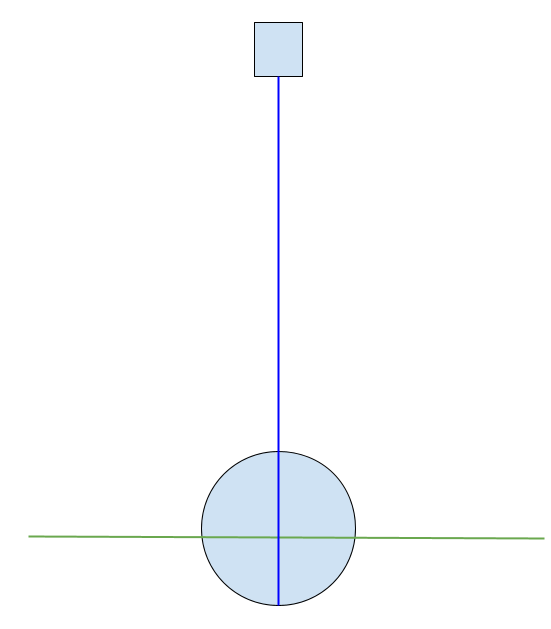
\includegraphics[width=0.4\linewidth]{../common/05_further_work/resources/00_genauigkeit_optimal.png}
    \caption{Optimale Genauigkeitsbestimmung}
    \label{fig:genauigkeit:optimal}
\end{figure}
Es ist offensichtlich, dass der Schnittpunkt des Strahls der Kamera aus mit der Ebene genau im Kugelzentrum liegt.
Wird nun angenommen, dass immer der reale Kugelmittelpunkt bestimmt werden kann, dann stimmt das Modell mit der Ebene
durch die Kugelzentren jedoch nicht mehr. Da die Kamera die Kugel aber immer weiter von der Seite sehen wird, je weiter diese am Rand
des Tischs liegt, wird diese zu einem Oval verzogen und es wird nicht mehr der reale Kugelmittelpunkt $M$ erkannt sondern ein Punkt $M'$
auf der Seite zur Kamera zugewandt. Das scheinbar optimale Verhalten sowie das reale ist in Abbildung \ref{fig:genauigkeit:real}
ersichtlich. Wie erkannt werden kann, ist die scheinbare Falscherkennung des Kugelmittelpunkts bei der Anwendung einer
Ebene auf Höhe des Kugelradius sogar von Vorteil, da die Fehlerdistanz zum realen Standort minimiert wird.
\begin{figure}[h!]
    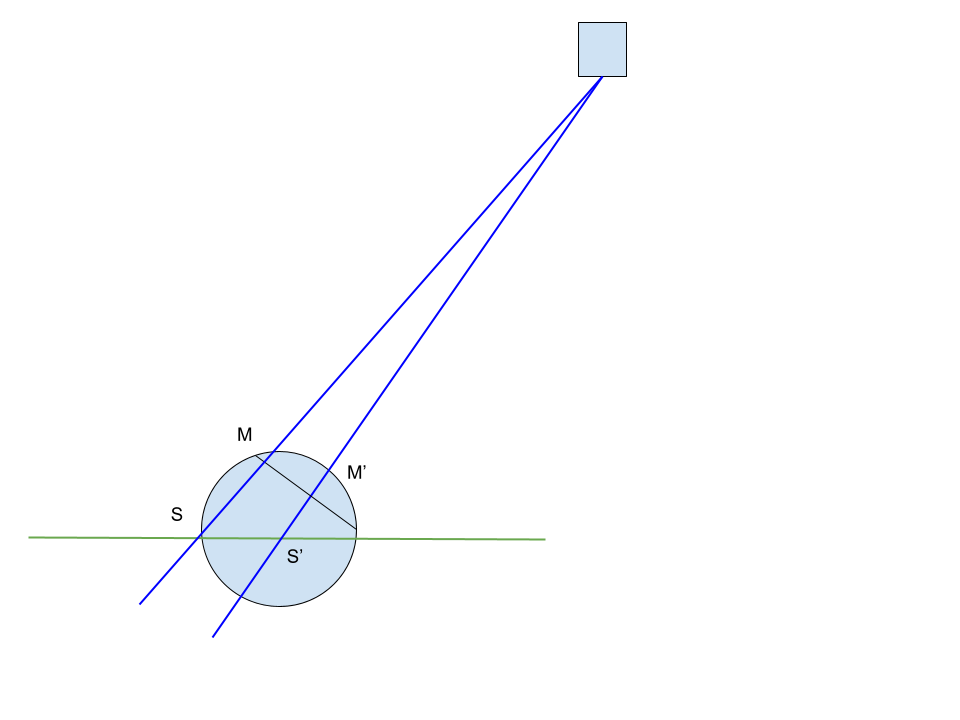
\includegraphics[width=0.4\linewidth]{../common/05_further_work/resources/01_genauigkeit_real.png}
    \caption{Reale Genauigkeitsbestimmung}
    \label{fig:genauigkeit:real}
\end{figure}


Nichtsdestotrotz kann es vonnöten sein, das Modell eventuell sogar der Realität entsprechend zu definieren, wenn erzielt
werden kann, dass immer der reale Kugelmittelpunkt gefunden wird. Weiterhin muss in diesem Zusammenhang zuerst ein genaueres
externes Messgerät gefunden werden, damit überhaupt eine Verbesserung der Genauigkeit nachgewiesen werden kann.


   \chapter{Weitere Arbeiten}
Die vorliegende Arbeit dient als Grundlage für die kommende Bachelor-Thesis. Daher gibt es diverse darauf aufbauende
Tätigkeiten. Diese sind unterschiedlich anspruchsvoll und ebenso von verschiedener Wichtigkeit. Daher werden
diese der Relevanz von definitiver Wichtigkeit bis potenzieller Wichtigkeit geordnet.
\section{Klassifikation der Kugeln}
In einem ersten Schritt muss die Klassifikation der Kugeln ergänzt werden. Hierbei geht es
um die Bestimmung der Art einer Kugel, ist es also eine Weisse, Rote oder Blaue. Als
Umsetzungshinweis sei hier der Hue-Kanal des Bildes gegeben.
\section{Erarbeitung des theoretischen physikalischen Modells}
Als Grundlage der Suche nach dem besten Stoss dient ein vereinfachtes theoretisches physikalisches
Modell. Dessen Parameter und Eigenschaften müssen bestimmt und in einen algorithmischen Kontext
verfasst werden. Hierbei sei angemerkt, dass eine Unmenge an möglichen Stössen betrachtet
werden müssen. Es muss also ein Konzept erarbeitet werden, das parallel jeweils nur
die besten Kandidaten verfolgt.
\section{Bestimmen der Heuristiken}
Zu einer erfolgreichen Suche gehört die Definition einer heuristischen Funktion, welche die
Optimalität eines Stosses wie auch dessen Resultat beschreibt. Dies setzt eine gewisse Kenntniss
über das Billardspiel voraus, wobei eventuell auf Wissen von Fachpersonen zugegriffen werden muss.
\section{Implementation der Suche}
Sobald das physikalische Modell, dessen Berechnungen sowie die Heuristiken stehen, kann die Suche
implementiert werden. Um das Vorgehen zu vereinfachen, wurde die Unity-Applikation bereits
entsprechend vorbereitet. Diese ist in der Lage, auf intuitive Weise verschiedenste Spielstatus zu
faken.
\newpage
\section{Verbesserung der Genauigkeit}
Sollte im Verlaufe der Entwicklung erkannt werden, dass die Präzision des Systems unzureichend
ist, kann diese über diverse Überlegungen eventuell verbessert werden. Eine bereits bekannte Problematik
stellt die Tatsache dar, dass eine Kugel, welche weit aussen am Tischrand liegt, von der Kamera oval gesehen wird.
Dies führt dazu, dass das Pixel, welches als Kugelmittelpunkt erkannt wird, nicht mit dem realen Mittelpunkt auf der Oberfläche übereinstimmt.
Dieses Problem wird jedoch durch die Art und Weise, wie der Standort der Kugel ermittelt wird, bereits ein wenig entschärft.
Die genaue Erläutering findet sich in Kapitel \ref{kap:camera_to_world}.
Es muss lediglich bekannt sein, dass der Standort durch einen Ray-Shoot von der Kamera aus durch den erkannten Kugelmittelpunkt
zu einer Ebene auf Höhe des Kugelradius bestimmt wird. Der Schnittpunkt mit dieser Ebene bildet die Position der Kugel. In einem optimalen Fall
wird jeweils der korrekte Kugelmittelpunkt erkannt. Dieses Szenario bildet auch die Grundlage für die Implementation und kann
aus Abbildung \ref{fig:genauigkeit:optimal} entnommen werden.
\begin{figure}[h!]
    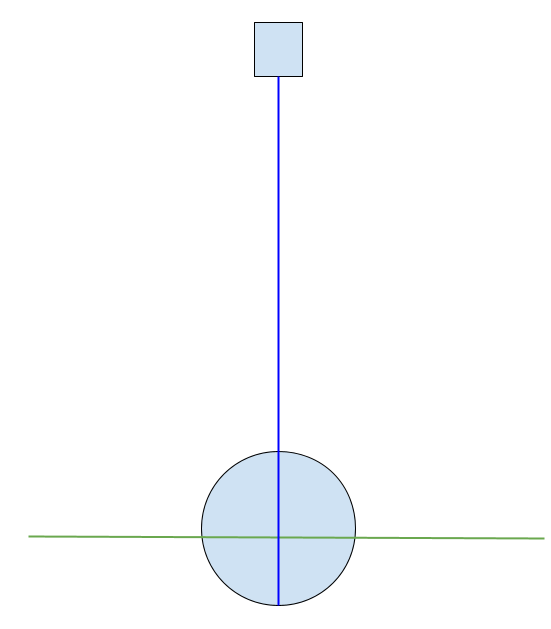
\includegraphics[width=0.4\linewidth]{../common/05_further_work/resources/00_genauigkeit_optimal.png}
    \caption{Optimale Genauigkeitsbestimmung}
    \label{fig:genauigkeit:optimal}
\end{figure}
Es ist offensichtlich, dass der Schnittpunkt des Strahls der Kamera aus mit der Ebene genau im Kugelzentrum liegt.
Wird nun angenommen, dass immer der reale Kugelmittelpunkt bestimmt werden kann, dann stimmt das Modell mit der Ebene
durch die Kugelzentren jedoch nicht mehr. Da die Kamera die Kugel aber immer weiter von der Seite sehen wird, je weiter diese am Rand
des Tischs liegt, wird diese zu einem Oval verzogen und es wird nicht mehr der reale Kugelmittelpunkt $M$ erkannt sondern ein Punkt $M'$
auf der Seite zur Kamera zugewandt. Das scheinbar optimale Verhalten sowie das reale ist in Abbildung \ref{fig:genauigkeit:real}
ersichtlich. Wie erkannt werden kann, ist die scheinbare Falscherkennung des Kugelmittelpunkts bei der Anwendung einer
Ebene auf Höhe des Kugelradius sogar von Vorteil, da die Fehlerdistanz zum realen Standort minimiert wird.
\begin{figure}[h!]
    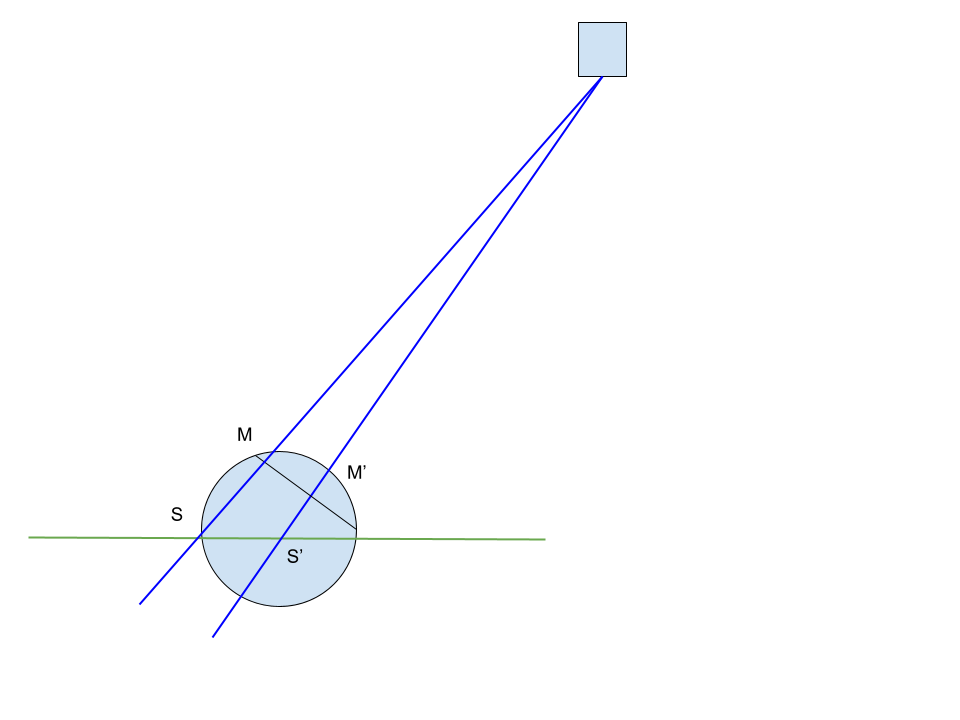
\includegraphics[width=0.4\linewidth]{../common/05_further_work/resources/01_genauigkeit_real.png}
    \caption{Reale Genauigkeitsbestimmung}
    \label{fig:genauigkeit:real}
\end{figure}


Nichtsdestotrotz kann es vonnöten sein, das Modell eventuell sogar der Realität entsprechend zu definieren, wenn erzielt
werden kann, dass immer der reale Kugelmittelpunkt gefunden wird. Weiterhin muss in diesem Zusammenhang zuerst ein genaueres
externes Messgerät gefunden werden, damit überhaupt eine Verbesserung der Genauigkeit nachgewiesen werden kann.


   \chapter{Weitere Arbeiten}
Die vorliegende Arbeit dient als Grundlage für die kommende Bachelor-Thesis. Daher gibt es diverse darauf aufbauende
Tätigkeiten. Diese sind unterschiedlich anspruchsvoll und ebenso von verschiedener Wichtigkeit. Daher werden
diese der Relevanz von definitiver Wichtigkeit bis potenzieller Wichtigkeit geordnet.
\section{Klassifikation der Kugeln}
In einem ersten Schritt muss die Klassifikation der Kugeln ergänzt werden. Hierbei geht es
um die Bestimmung der Art einer Kugel, ist es also eine Weisse, Rote oder Blaue. Als
Umsetzungshinweis sei hier der Hue-Kanal des Bildes gegeben.
\section{Erarbeitung des theoretischen physikalischen Modells}
Als Grundlage der Suche nach dem besten Stoss dient ein vereinfachtes theoretisches physikalisches
Modell. Dessen Parameter und Eigenschaften müssen bestimmt und in einen algorithmischen Kontext
verfasst werden. Hierbei sei angemerkt, dass eine Unmenge an möglichen Stössen betrachtet
werden müssen. Es muss also ein Konzept erarbeitet werden, das parallel jeweils nur
die besten Kandidaten verfolgt.
\section{Bestimmen der Heuristiken}
Zu einer erfolgreichen Suche gehört die Definition einer heuristischen Funktion, welche die
Optimalität eines Stosses wie auch dessen Resultat beschreibt. Dies setzt eine gewisse Kenntniss
über das Billardspiel voraus, wobei eventuell auf Wissen von Fachpersonen zugegriffen werden muss.
\section{Implementation der Suche}
Sobald das physikalische Modell, dessen Berechnungen sowie die Heuristiken stehen, kann die Suche
implementiert werden. Um das Vorgehen zu vereinfachen, wurde die Unity-Applikation bereits
entsprechend vorbereitet. Diese ist in der Lage, auf intuitive Weise verschiedenste Spielstatus zu
faken.
\newpage
\section{Verbesserung der Genauigkeit}
Sollte im Verlaufe der Entwicklung erkannt werden, dass die Präzision des Systems unzureichend
ist, kann diese über diverse Überlegungen eventuell verbessert werden. Eine bereits bekannte Problematik
stellt die Tatsache dar, dass eine Kugel, welche weit aussen am Tischrand liegt, von der Kamera oval gesehen wird.
Dies führt dazu, dass das Pixel, welches als Kugelmittelpunkt erkannt wird, nicht mit dem realen Mittelpunkt auf der Oberfläche übereinstimmt.
Dieses Problem wird jedoch durch die Art und Weise, wie der Standort der Kugel ermittelt wird, bereits ein wenig entschärft.
Die genaue Erläutering findet sich in Kapitel \ref{kap:camera_to_world}.
Es muss lediglich bekannt sein, dass der Standort durch einen Ray-Shoot von der Kamera aus durch den erkannten Kugelmittelpunkt
zu einer Ebene auf Höhe des Kugelradius bestimmt wird. Der Schnittpunkt mit dieser Ebene bildet die Position der Kugel. In einem optimalen Fall
wird jeweils der korrekte Kugelmittelpunkt erkannt. Dieses Szenario bildet auch die Grundlage für die Implementation und kann
aus Abbildung \ref{fig:genauigkeit:optimal} entnommen werden.
\begin{figure}[h!]
    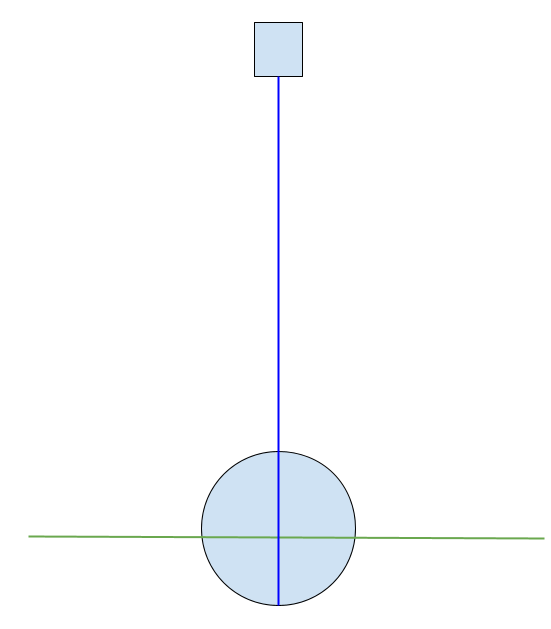
\includegraphics[width=0.4\linewidth]{../common/05_further_work/resources/00_genauigkeit_optimal.png}
    \caption{Optimale Genauigkeitsbestimmung}
    \label{fig:genauigkeit:optimal}
\end{figure}
Es ist offensichtlich, dass der Schnittpunkt des Strahls der Kamera aus mit der Ebene genau im Kugelzentrum liegt.
Wird nun angenommen, dass immer der reale Kugelmittelpunkt bestimmt werden kann, dann stimmt das Modell mit der Ebene
durch die Kugelzentren jedoch nicht mehr. Da die Kamera die Kugel aber immer weiter von der Seite sehen wird, je weiter diese am Rand
des Tischs liegt, wird diese zu einem Oval verzogen und es wird nicht mehr der reale Kugelmittelpunkt $M$ erkannt sondern ein Punkt $M'$
auf der Seite zur Kamera zugewandt. Das scheinbar optimale Verhalten sowie das reale ist in Abbildung \ref{fig:genauigkeit:real}
ersichtlich. Wie erkannt werden kann, ist die scheinbare Falscherkennung des Kugelmittelpunkts bei der Anwendung einer
Ebene auf Höhe des Kugelradius sogar von Vorteil, da die Fehlerdistanz zum realen Standort minimiert wird.
\begin{figure}[h!]
    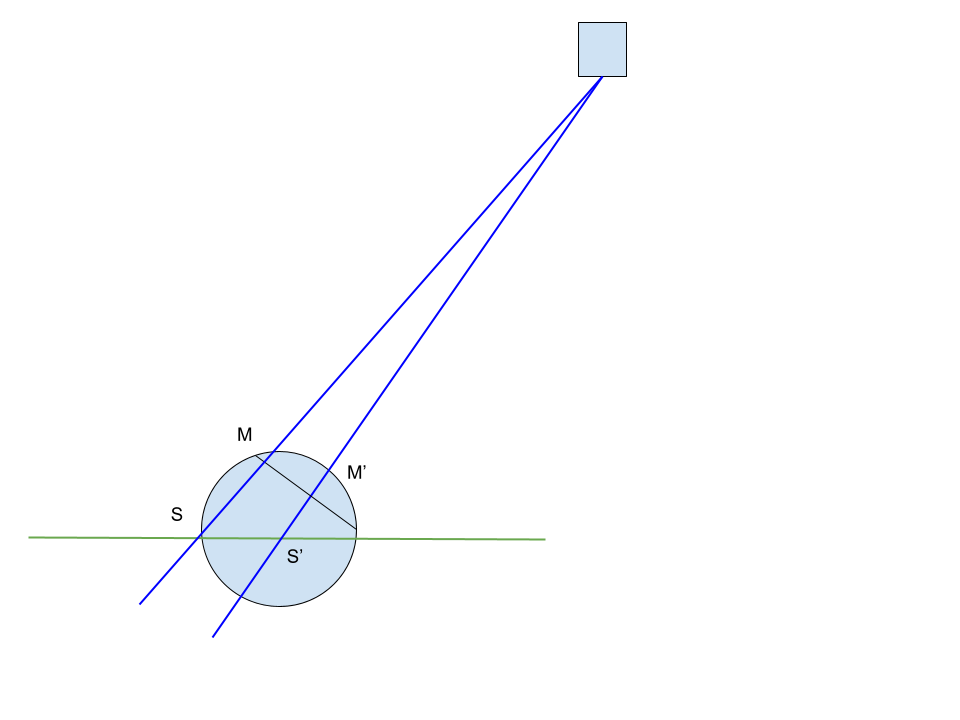
\includegraphics[width=0.4\linewidth]{../common/05_further_work/resources/01_genauigkeit_real.png}
    \caption{Reale Genauigkeitsbestimmung}
    \label{fig:genauigkeit:real}
\end{figure}


Nichtsdestotrotz kann es vonnöten sein, das Modell eventuell sogar der Realität entsprechend zu definieren, wenn erzielt
werden kann, dass immer der reale Kugelmittelpunkt gefunden wird. Weiterhin muss in diesem Zusammenhang zuerst ein genaueres
externes Messgerät gefunden werden, damit überhaupt eine Verbesserung der Genauigkeit nachgewiesen werden kann.


   \chapter{Weitere Arbeiten}
Die vorliegende Arbeit dient als Grundlage für die kommende Bachelor-Thesis. Daher gibt es diverse darauf aufbauende
Tätigkeiten. Diese sind unterschiedlich anspruchsvoll und ebenso von verschiedener Wichtigkeit. Daher werden
diese der Relevanz von definitiver Wichtigkeit bis potenzieller Wichtigkeit geordnet.
\section{Klassifikation der Kugeln}
In einem ersten Schritt muss die Klassifikation der Kugeln ergänzt werden. Hierbei geht es
um die Bestimmung der Art einer Kugel, ist es also eine Weisse, Rote oder Blaue. Als
Umsetzungshinweis sei hier der Hue-Kanal des Bildes gegeben.
\section{Erarbeitung des theoretischen physikalischen Modells}
Als Grundlage der Suche nach dem besten Stoss dient ein vereinfachtes theoretisches physikalisches
Modell. Dessen Parameter und Eigenschaften müssen bestimmt und in einen algorithmischen Kontext
verfasst werden. Hierbei sei angemerkt, dass eine Unmenge an möglichen Stössen betrachtet
werden müssen. Es muss also ein Konzept erarbeitet werden, das parallel jeweils nur
die besten Kandidaten verfolgt.
\section{Bestimmen der Heuristiken}
Zu einer erfolgreichen Suche gehört die Definition einer heuristischen Funktion, welche die
Optimalität eines Stosses wie auch dessen Resultat beschreibt. Dies setzt eine gewisse Kenntniss
über das Billardspiel voraus, wobei eventuell auf Wissen von Fachpersonen zugegriffen werden muss.
\section{Implementation der Suche}
Sobald das physikalische Modell, dessen Berechnungen sowie die Heuristiken stehen, kann die Suche
implementiert werden. Um das Vorgehen zu vereinfachen, wurde die Unity-Applikation bereits
entsprechend vorbereitet. Diese ist in der Lage, auf intuitive Weise verschiedenste Spielstatus zu
faken.
\newpage
\section{Verbesserung der Genauigkeit}
Sollte im Verlaufe der Entwicklung erkannt werden, dass die Präzision des Systems unzureichend
ist, kann diese über diverse Überlegungen eventuell verbessert werden. Eine bereits bekannte Problematik
stellt die Tatsache dar, dass eine Kugel, welche weit aussen am Tischrand liegt, von der Kamera oval gesehen wird.
Dies führt dazu, dass das Pixel, welches als Kugelmittelpunkt erkannt wird, nicht mit dem realen Mittelpunkt auf der Oberfläche übereinstimmt.
Dieses Problem wird jedoch durch die Art und Weise, wie der Standort der Kugel ermittelt wird, bereits ein wenig entschärft.
Die genaue Erläutering findet sich in Kapitel \ref{kap:camera_to_world}.
Es muss lediglich bekannt sein, dass der Standort durch einen Ray-Shoot von der Kamera aus durch den erkannten Kugelmittelpunkt
zu einer Ebene auf Höhe des Kugelradius bestimmt wird. Der Schnittpunkt mit dieser Ebene bildet die Position der Kugel. In einem optimalen Fall
wird jeweils der korrekte Kugelmittelpunkt erkannt. Dieses Szenario bildet auch die Grundlage für die Implementation und kann
aus Abbildung \ref{fig:genauigkeit:optimal} entnommen werden.
\begin{figure}[h!]
    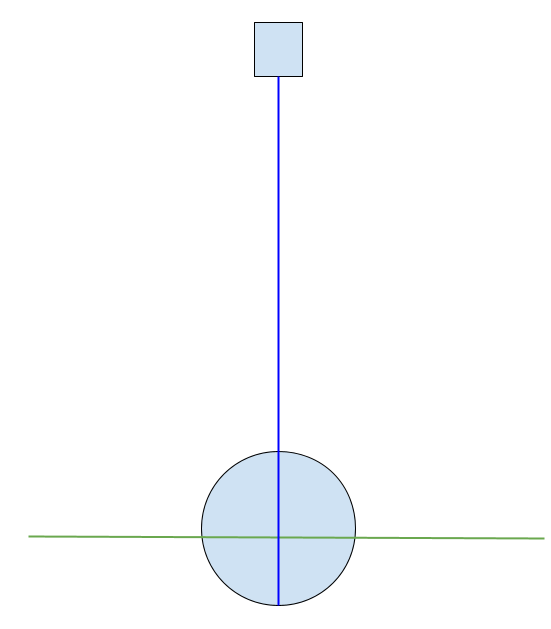
\includegraphics[width=0.4\linewidth]{../common/05_further_work/resources/00_genauigkeit_optimal.png}
    \caption{Optimale Genauigkeitsbestimmung}
    \label{fig:genauigkeit:optimal}
\end{figure}
Es ist offensichtlich, dass der Schnittpunkt des Strahls der Kamera aus mit der Ebene genau im Kugelzentrum liegt.
Wird nun angenommen, dass immer der reale Kugelmittelpunkt bestimmt werden kann, dann stimmt das Modell mit der Ebene
durch die Kugelzentren jedoch nicht mehr. Da die Kamera die Kugel aber immer weiter von der Seite sehen wird, je weiter diese am Rand
des Tischs liegt, wird diese zu einem Oval verzogen und es wird nicht mehr der reale Kugelmittelpunkt $M$ erkannt sondern ein Punkt $M'$
auf der Seite zur Kamera zugewandt. Das scheinbar optimale Verhalten sowie das reale ist in Abbildung \ref{fig:genauigkeit:real}
ersichtlich. Wie erkannt werden kann, ist die scheinbare Falscherkennung des Kugelmittelpunkts bei der Anwendung einer
Ebene auf Höhe des Kugelradius sogar von Vorteil, da die Fehlerdistanz zum realen Standort minimiert wird.
\begin{figure}[h!]
    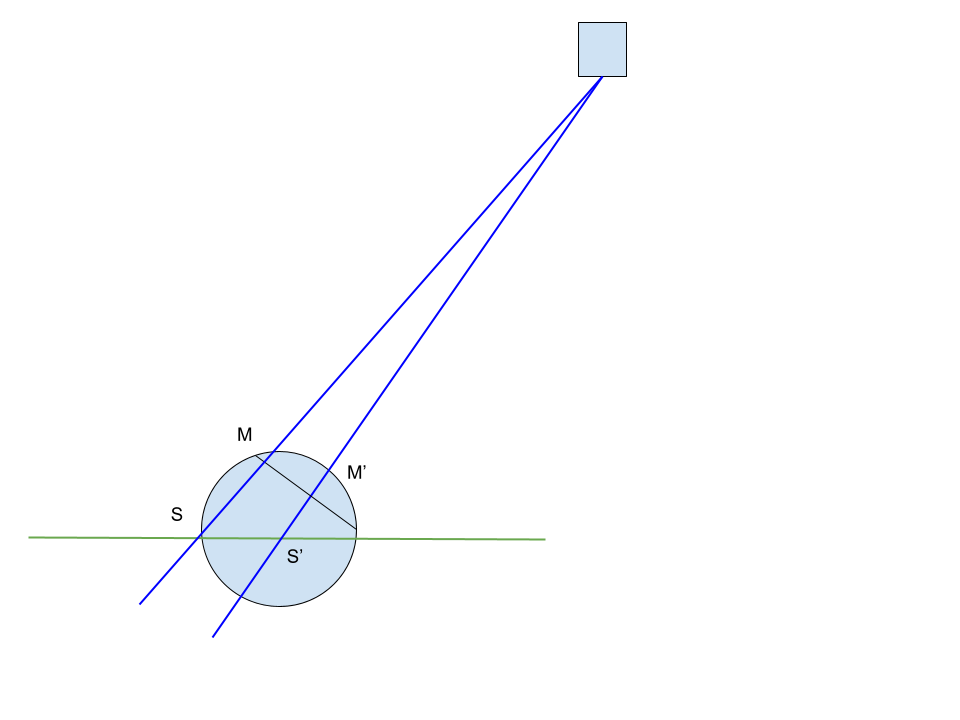
\includegraphics[width=0.4\linewidth]{../common/05_further_work/resources/01_genauigkeit_real.png}
    \caption{Reale Genauigkeitsbestimmung}
    \label{fig:genauigkeit:real}
\end{figure}


Nichtsdestotrotz kann es vonnöten sein, das Modell eventuell sogar der Realität entsprechend zu definieren, wenn erzielt
werden kann, dass immer der reale Kugelmittelpunkt gefunden wird. Weiterhin muss in diesem Zusammenhang zuerst ein genaueres
externes Messgerät gefunden werden, damit überhaupt eine Verbesserung der Genauigkeit nachgewiesen werden kann.


   \chapter{Weitere Arbeiten}
Die vorliegende Arbeit dient als Grundlage für die kommende Bachelor-Thesis. Daher gibt es diverse darauf aufbauende
Tätigkeiten. Diese sind unterschiedlich anspruchsvoll und ebenso von verschiedener Wichtigkeit. Daher werden
diese der Relevanz von definitiver Wichtigkeit bis potenzieller Wichtigkeit geordnet.
\section{Klassifikation der Kugeln}
In einem ersten Schritt muss die Klassifikation der Kugeln ergänzt werden. Hierbei geht es
um die Bestimmung der Art einer Kugel, ist es also eine Weisse, Rote oder Blaue. Als
Umsetzungshinweis sei hier der Hue-Kanal des Bildes gegeben.
\section{Erarbeitung des theoretischen physikalischen Modells}
Als Grundlage der Suche nach dem besten Stoss dient ein vereinfachtes theoretisches physikalisches
Modell. Dessen Parameter und Eigenschaften müssen bestimmt und in einen algorithmischen Kontext
verfasst werden. Hierbei sei angemerkt, dass eine Unmenge an möglichen Stössen betrachtet
werden müssen. Es muss also ein Konzept erarbeitet werden, das parallel jeweils nur
die besten Kandidaten verfolgt.
\section{Bestimmen der Heuristiken}
Zu einer erfolgreichen Suche gehört die Definition einer heuristischen Funktion, welche die
Optimalität eines Stosses wie auch dessen Resultat beschreibt. Dies setzt eine gewisse Kenntniss
über das Billardspiel voraus, wobei eventuell auf Wissen von Fachpersonen zugegriffen werden muss.
\section{Implementation der Suche}
Sobald das physikalische Modell, dessen Berechnungen sowie die Heuristiken stehen, kann die Suche
implementiert werden. Um das Vorgehen zu vereinfachen, wurde die Unity-Applikation bereits
entsprechend vorbereitet. Diese ist in der Lage, auf intuitive Weise verschiedenste Spielstatus zu
faken.
\newpage
\section{Verbesserung der Genauigkeit}
Sollte im Verlaufe der Entwicklung erkannt werden, dass die Präzision des Systems unzureichend
ist, kann diese über diverse Überlegungen eventuell verbessert werden. Eine bereits bekannte Problematik
stellt die Tatsache dar, dass eine Kugel, welche weit aussen am Tischrand liegt, von der Kamera oval gesehen wird.
Dies führt dazu, dass das Pixel, welches als Kugelmittelpunkt erkannt wird, nicht mit dem realen Mittelpunkt auf der Oberfläche übereinstimmt.
Dieses Problem wird jedoch durch die Art und Weise, wie der Standort der Kugel ermittelt wird, bereits ein wenig entschärft.
Die genaue Erläutering findet sich in Kapitel \ref{kap:camera_to_world}.
Es muss lediglich bekannt sein, dass der Standort durch einen Ray-Shoot von der Kamera aus durch den erkannten Kugelmittelpunkt
zu einer Ebene auf Höhe des Kugelradius bestimmt wird. Der Schnittpunkt mit dieser Ebene bildet die Position der Kugel. In einem optimalen Fall
wird jeweils der korrekte Kugelmittelpunkt erkannt. Dieses Szenario bildet auch die Grundlage für die Implementation und kann
aus Abbildung \ref{fig:genauigkeit:optimal} entnommen werden.
\begin{figure}[h!]
    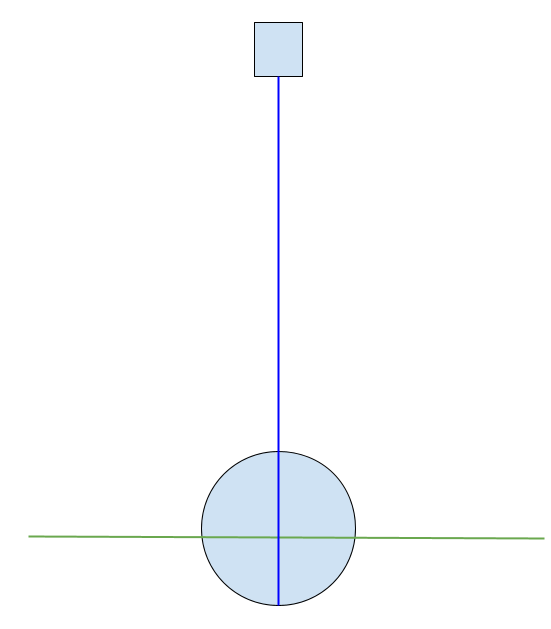
\includegraphics[width=0.4\linewidth]{../common/05_further_work/resources/00_genauigkeit_optimal.png}
    \caption{Optimale Genauigkeitsbestimmung}
    \label{fig:genauigkeit:optimal}
\end{figure}
Es ist offensichtlich, dass der Schnittpunkt des Strahls der Kamera aus mit der Ebene genau im Kugelzentrum liegt.
Wird nun angenommen, dass immer der reale Kugelmittelpunkt bestimmt werden kann, dann stimmt das Modell mit der Ebene
durch die Kugelzentren jedoch nicht mehr. Da die Kamera die Kugel aber immer weiter von der Seite sehen wird, je weiter diese am Rand
des Tischs liegt, wird diese zu einem Oval verzogen und es wird nicht mehr der reale Kugelmittelpunkt $M$ erkannt sondern ein Punkt $M'$
auf der Seite zur Kamera zugewandt. Das scheinbar optimale Verhalten sowie das reale ist in Abbildung \ref{fig:genauigkeit:real}
ersichtlich. Wie erkannt werden kann, ist die scheinbare Falscherkennung des Kugelmittelpunkts bei der Anwendung einer
Ebene auf Höhe des Kugelradius sogar von Vorteil, da die Fehlerdistanz zum realen Standort minimiert wird.
\begin{figure}[h!]
    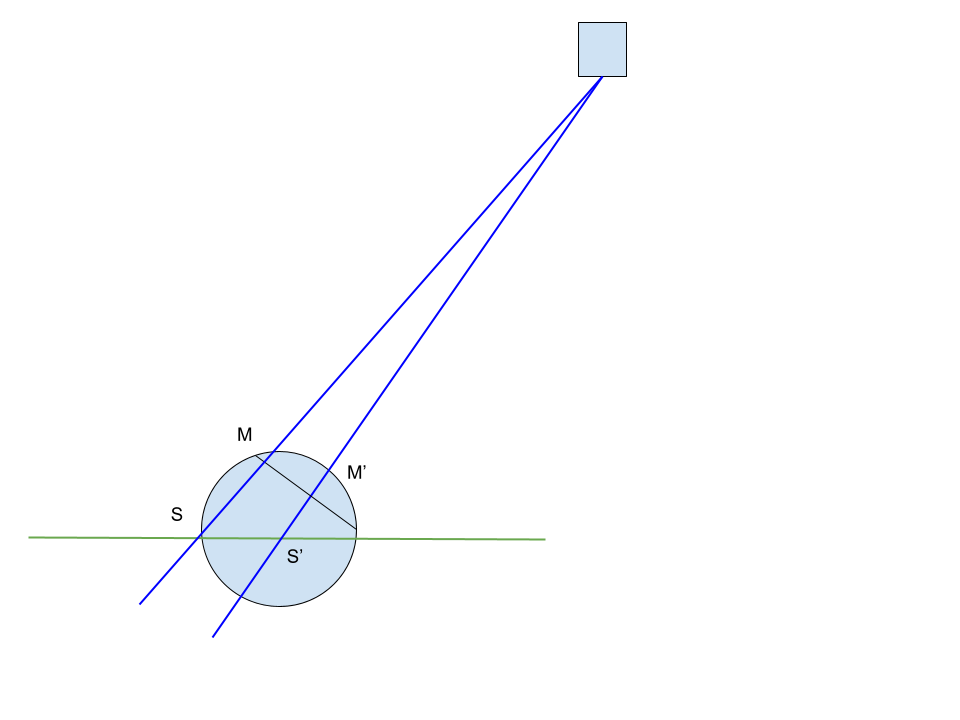
\includegraphics[width=0.4\linewidth]{../common/05_further_work/resources/01_genauigkeit_real.png}
    \caption{Reale Genauigkeitsbestimmung}
    \label{fig:genauigkeit:real}
\end{figure}


Nichtsdestotrotz kann es vonnöten sein, das Modell eventuell sogar der Realität entsprechend zu definieren, wenn erzielt
werden kann, dass immer der reale Kugelmittelpunkt gefunden wird. Weiterhin muss in diesem Zusammenhang zuerst ein genaueres
externes Messgerät gefunden werden, damit überhaupt eine Verbesserung der Genauigkeit nachgewiesen werden kann.


   \chapter{Weitere Arbeiten}
Die vorliegende Arbeit dient als Grundlage für die kommende Bachelor-Thesis. Daher gibt es diverse darauf aufbauende
Tätigkeiten. Diese sind unterschiedlich anspruchsvoll und ebenso von verschiedener Wichtigkeit. Daher werden
diese der Relevanz von definitiver Wichtigkeit bis potenzieller Wichtigkeit geordnet.
\section{Klassifikation der Kugeln}
In einem ersten Schritt muss die Klassifikation der Kugeln ergänzt werden. Hierbei geht es
um die Bestimmung der Art einer Kugel, ist es also eine Weisse, Rote oder Blaue. Als
Umsetzungshinweis sei hier der Hue-Kanal des Bildes gegeben.
\section{Erarbeitung des theoretischen physikalischen Modells}
Als Grundlage der Suche nach dem besten Stoss dient ein vereinfachtes theoretisches physikalisches
Modell. Dessen Parameter und Eigenschaften müssen bestimmt und in einen algorithmischen Kontext
verfasst werden. Hierbei sei angemerkt, dass eine Unmenge an möglichen Stössen betrachtet
werden müssen. Es muss also ein Konzept erarbeitet werden, das parallel jeweils nur
die besten Kandidaten verfolgt.
\section{Bestimmen der Heuristiken}
Zu einer erfolgreichen Suche gehört die Definition einer heuristischen Funktion, welche die
Optimalität eines Stosses wie auch dessen Resultat beschreibt. Dies setzt eine gewisse Kenntniss
über das Billardspiel voraus, wobei eventuell auf Wissen von Fachpersonen zugegriffen werden muss.
\section{Implementation der Suche}
Sobald das physikalische Modell, dessen Berechnungen sowie die Heuristiken stehen, kann die Suche
implementiert werden. Um das Vorgehen zu vereinfachen, wurde die Unity-Applikation bereits
entsprechend vorbereitet. Diese ist in der Lage, auf intuitive Weise verschiedenste Spielstatus zu
faken.
\newpage
\section{Verbesserung der Genauigkeit}
Sollte im Verlaufe der Entwicklung erkannt werden, dass die Präzision des Systems unzureichend
ist, kann diese über diverse Überlegungen eventuell verbessert werden. Eine bereits bekannte Problematik
stellt die Tatsache dar, dass eine Kugel, welche weit aussen am Tischrand liegt, von der Kamera oval gesehen wird.
Dies führt dazu, dass das Pixel, welches als Kugelmittelpunkt erkannt wird, nicht mit dem realen Mittelpunkt auf der Oberfläche übereinstimmt.
Dieses Problem wird jedoch durch die Art und Weise, wie der Standort der Kugel ermittelt wird, bereits ein wenig entschärft.
Die genaue Erläutering findet sich in Kapitel \ref{kap:camera_to_world}.
Es muss lediglich bekannt sein, dass der Standort durch einen Ray-Shoot von der Kamera aus durch den erkannten Kugelmittelpunkt
zu einer Ebene auf Höhe des Kugelradius bestimmt wird. Der Schnittpunkt mit dieser Ebene bildet die Position der Kugel. In einem optimalen Fall
wird jeweils der korrekte Kugelmittelpunkt erkannt. Dieses Szenario bildet auch die Grundlage für die Implementation und kann
aus Abbildung \ref{fig:genauigkeit:optimal} entnommen werden.
\begin{figure}[h!]
    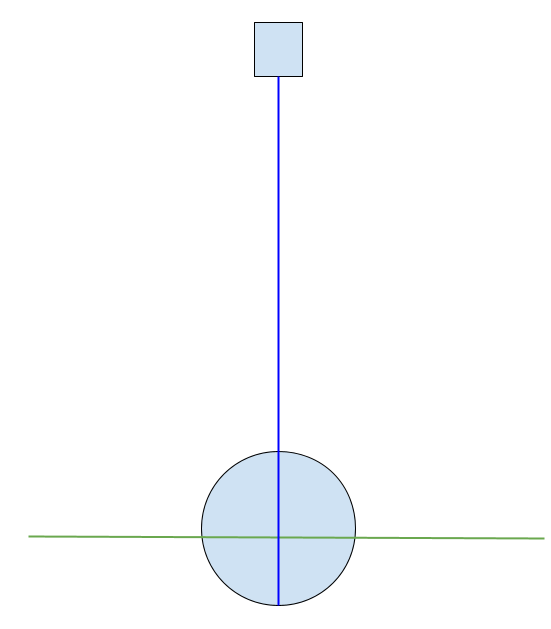
\includegraphics[width=0.4\linewidth]{../common/05_further_work/resources/00_genauigkeit_optimal.png}
    \caption{Optimale Genauigkeitsbestimmung}
    \label{fig:genauigkeit:optimal}
\end{figure}
Es ist offensichtlich, dass der Schnittpunkt des Strahls der Kamera aus mit der Ebene genau im Kugelzentrum liegt.
Wird nun angenommen, dass immer der reale Kugelmittelpunkt bestimmt werden kann, dann stimmt das Modell mit der Ebene
durch die Kugelzentren jedoch nicht mehr. Da die Kamera die Kugel aber immer weiter von der Seite sehen wird, je weiter diese am Rand
des Tischs liegt, wird diese zu einem Oval verzogen und es wird nicht mehr der reale Kugelmittelpunkt $M$ erkannt sondern ein Punkt $M'$
auf der Seite zur Kamera zugewandt. Das scheinbar optimale Verhalten sowie das reale ist in Abbildung \ref{fig:genauigkeit:real}
ersichtlich. Wie erkannt werden kann, ist die scheinbare Falscherkennung des Kugelmittelpunkts bei der Anwendung einer
Ebene auf Höhe des Kugelradius sogar von Vorteil, da die Fehlerdistanz zum realen Standort minimiert wird.
\begin{figure}[h!]
    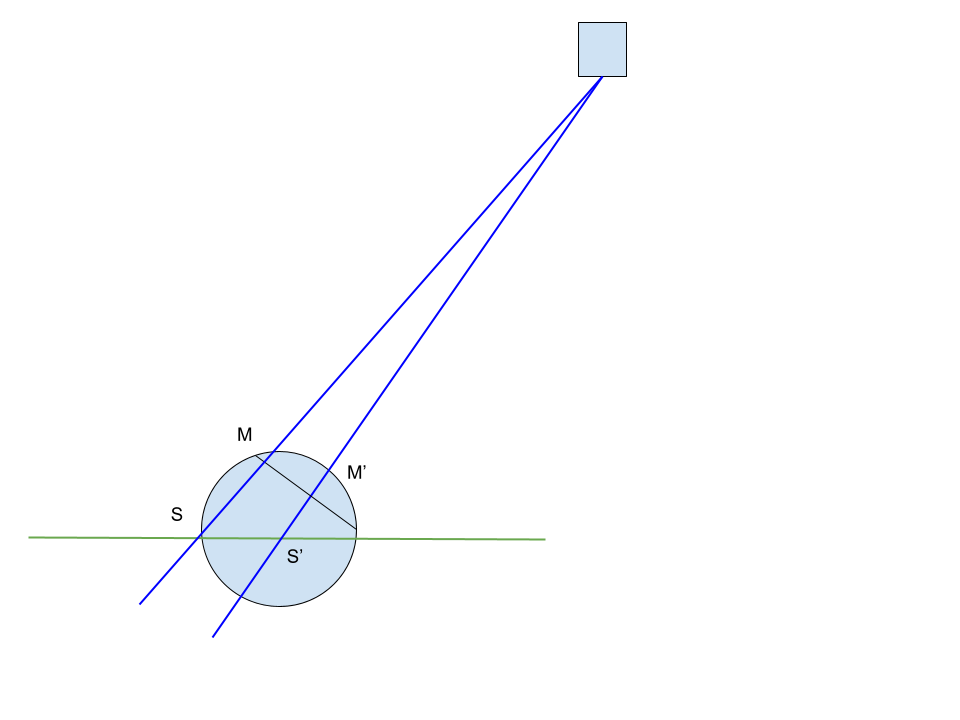
\includegraphics[width=0.4\linewidth]{../common/05_further_work/resources/01_genauigkeit_real.png}
    \caption{Reale Genauigkeitsbestimmung}
    \label{fig:genauigkeit:real}
\end{figure}


Nichtsdestotrotz kann es vonnöten sein, das Modell eventuell sogar der Realität entsprechend zu definieren, wenn erzielt
werden kann, dass immer der reale Kugelmittelpunkt gefunden wird. Weiterhin muss in diesem Zusammenhang zuerst ein genaueres
externes Messgerät gefunden werden, damit überhaupt eine Verbesserung der Genauigkeit nachgewiesen werden kann.


   \chapter{Weitere Arbeiten}
Die vorliegende Arbeit dient als Grundlage für die kommende Bachelor-Thesis. Daher gibt es diverse darauf aufbauende
Tätigkeiten. Diese sind unterschiedlich anspruchsvoll und ebenso von verschiedener Wichtigkeit. Daher werden
diese der Relevanz von definitiver Wichtigkeit bis potenzieller Wichtigkeit geordnet.
\section{Klassifikation der Kugeln}
In einem ersten Schritt muss die Klassifikation der Kugeln ergänzt werden. Hierbei geht es
um die Bestimmung der Art einer Kugel, ist es also eine Weisse, Rote oder Blaue. Als
Umsetzungshinweis sei hier der Hue-Kanal des Bildes gegeben.
\section{Erarbeitung des theoretischen physikalischen Modells}
Als Grundlage der Suche nach dem besten Stoss dient ein vereinfachtes theoretisches physikalisches
Modell. Dessen Parameter und Eigenschaften müssen bestimmt und in einen algorithmischen Kontext
verfasst werden. Hierbei sei angemerkt, dass eine Unmenge an möglichen Stössen betrachtet
werden müssen. Es muss also ein Konzept erarbeitet werden, das parallel jeweils nur
die besten Kandidaten verfolgt.
\section{Bestimmen der Heuristiken}
Zu einer erfolgreichen Suche gehört die Definition einer heuristischen Funktion, welche die
Optimalität eines Stosses wie auch dessen Resultat beschreibt. Dies setzt eine gewisse Kenntniss
über das Billardspiel voraus, wobei eventuell auf Wissen von Fachpersonen zugegriffen werden muss.
\section{Implementation der Suche}
Sobald das physikalische Modell, dessen Berechnungen sowie die Heuristiken stehen, kann die Suche
implementiert werden. Um das Vorgehen zu vereinfachen, wurde die Unity-Applikation bereits
entsprechend vorbereitet. Diese ist in der Lage, auf intuitive Weise verschiedenste Spielstatus zu
faken.
\newpage
\section{Verbesserung der Genauigkeit}
Sollte im Verlaufe der Entwicklung erkannt werden, dass die Präzision des Systems unzureichend
ist, kann diese über diverse Überlegungen eventuell verbessert werden. Eine bereits bekannte Problematik
stellt die Tatsache dar, dass eine Kugel, welche weit aussen am Tischrand liegt, von der Kamera oval gesehen wird.
Dies führt dazu, dass das Pixel, welches als Kugelmittelpunkt erkannt wird, nicht mit dem realen Mittelpunkt auf der Oberfläche übereinstimmt.
Dieses Problem wird jedoch durch die Art und Weise, wie der Standort der Kugel ermittelt wird, bereits ein wenig entschärft.
Die genaue Erläutering findet sich in Kapitel \ref{kap:camera_to_world}.
Es muss lediglich bekannt sein, dass der Standort durch einen Ray-Shoot von der Kamera aus durch den erkannten Kugelmittelpunkt
zu einer Ebene auf Höhe des Kugelradius bestimmt wird. Der Schnittpunkt mit dieser Ebene bildet die Position der Kugel. In einem optimalen Fall
wird jeweils der korrekte Kugelmittelpunkt erkannt. Dieses Szenario bildet auch die Grundlage für die Implementation und kann
aus Abbildung \ref{fig:genauigkeit:optimal} entnommen werden.
\begin{figure}[h!]
    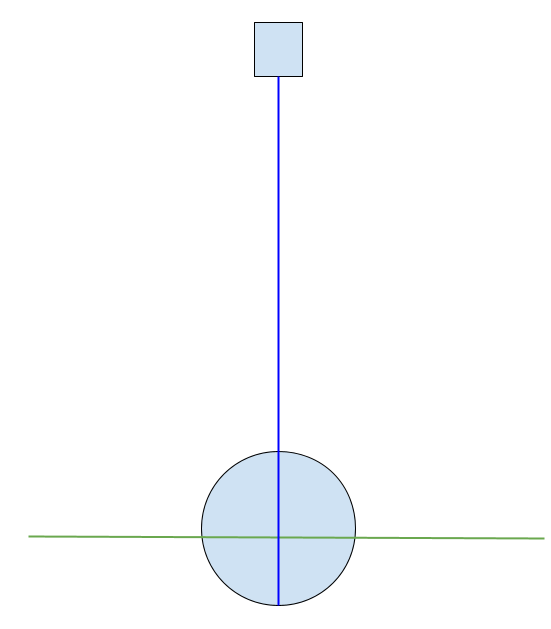
\includegraphics[width=0.4\linewidth]{../common/05_further_work/resources/00_genauigkeit_optimal.png}
    \caption{Optimale Genauigkeitsbestimmung}
    \label{fig:genauigkeit:optimal}
\end{figure}
Es ist offensichtlich, dass der Schnittpunkt des Strahls der Kamera aus mit der Ebene genau im Kugelzentrum liegt.
Wird nun angenommen, dass immer der reale Kugelmittelpunkt bestimmt werden kann, dann stimmt das Modell mit der Ebene
durch die Kugelzentren jedoch nicht mehr. Da die Kamera die Kugel aber immer weiter von der Seite sehen wird, je weiter diese am Rand
des Tischs liegt, wird diese zu einem Oval verzogen und es wird nicht mehr der reale Kugelmittelpunkt $M$ erkannt sondern ein Punkt $M'$
auf der Seite zur Kamera zugewandt. Das scheinbar optimale Verhalten sowie das reale ist in Abbildung \ref{fig:genauigkeit:real}
ersichtlich. Wie erkannt werden kann, ist die scheinbare Falscherkennung des Kugelmittelpunkts bei der Anwendung einer
Ebene auf Höhe des Kugelradius sogar von Vorteil, da die Fehlerdistanz zum realen Standort minimiert wird.
\begin{figure}[h!]
    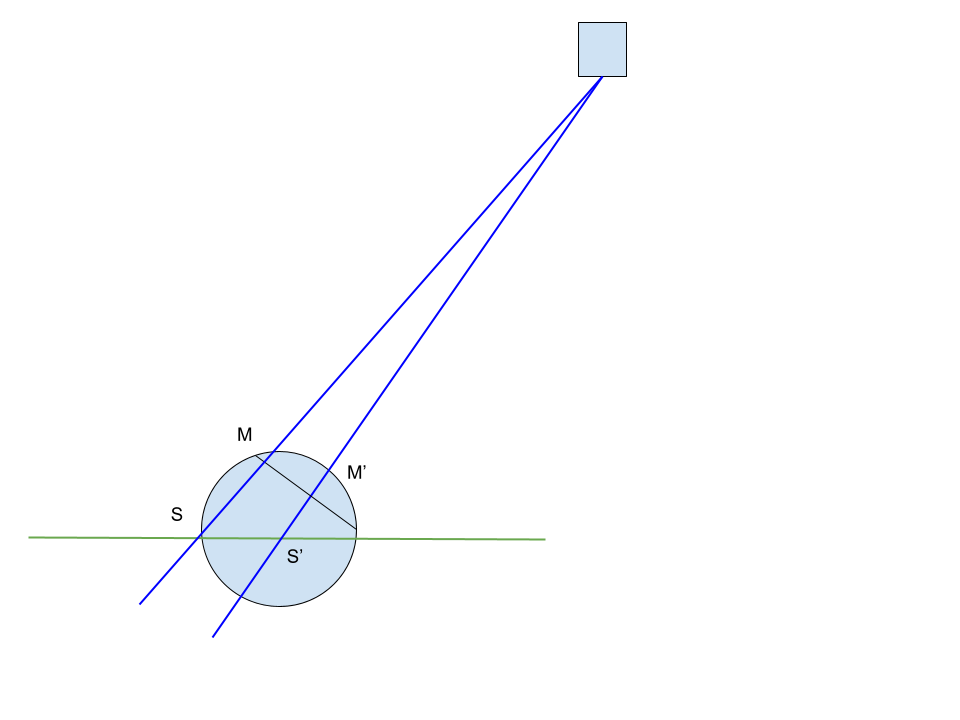
\includegraphics[width=0.4\linewidth]{../common/05_further_work/resources/01_genauigkeit_real.png}
    \caption{Reale Genauigkeitsbestimmung}
    \label{fig:genauigkeit:real}
\end{figure}


Nichtsdestotrotz kann es vonnöten sein, das Modell eventuell sogar der Realität entsprechend zu definieren, wenn erzielt
werden kann, dass immer der reale Kugelmittelpunkt gefunden wird. Weiterhin muss in diesem Zusammenhang zuerst ein genaueres
externes Messgerät gefunden werden, damit überhaupt eine Verbesserung der Genauigkeit nachgewiesen werden kann.



% List of Figures
    \listoffigures
% List of Tables
    \listoftables
% Bibliography
    \printbibliography
% Glossary
%    \printunsrtglossary[style={index}]

    
\includepdf[pages=-]{../common/resources/01_erklaerung.pdf}
    
\includepdf[pages=-]{../common/resources/01_erklaerung.pdf}

% Appendices
    \chapter{Weitere Arbeiten}
Die vorliegende Arbeit dient als Grundlage für die kommende Bachelor-Thesis. Daher gibt es diverse darauf aufbauende
Tätigkeiten. Diese sind unterschiedlich anspruchsvoll und ebenso von verschiedener Wichtigkeit. Daher werden
diese der Relevanz von definitiver Wichtigkeit bis potenzieller Wichtigkeit geordnet.
\section{Klassifikation der Kugeln}
In einem ersten Schritt muss die Klassifikation der Kugeln ergänzt werden. Hierbei geht es
um die Bestimmung der Art einer Kugel, ist es also eine Weisse, Rote oder Blaue. Als
Umsetzungshinweis sei hier der Hue-Kanal des Bildes gegeben.
\section{Erarbeitung des theoretischen physikalischen Modells}
Als Grundlage der Suche nach dem besten Stoss dient ein vereinfachtes theoretisches physikalisches
Modell. Dessen Parameter und Eigenschaften müssen bestimmt und in einen algorithmischen Kontext
verfasst werden. Hierbei sei angemerkt, dass eine Unmenge an möglichen Stössen betrachtet
werden müssen. Es muss also ein Konzept erarbeitet werden, das parallel jeweils nur
die besten Kandidaten verfolgt.
\section{Bestimmen der Heuristiken}
Zu einer erfolgreichen Suche gehört die Definition einer heuristischen Funktion, welche die
Optimalität eines Stosses wie auch dessen Resultat beschreibt. Dies setzt eine gewisse Kenntniss
über das Billardspiel voraus, wobei eventuell auf Wissen von Fachpersonen zugegriffen werden muss.
\section{Implementation der Suche}
Sobald das physikalische Modell, dessen Berechnungen sowie die Heuristiken stehen, kann die Suche
implementiert werden. Um das Vorgehen zu vereinfachen, wurde die Unity-Applikation bereits
entsprechend vorbereitet. Diese ist in der Lage, auf intuitive Weise verschiedenste Spielstatus zu
faken.
\newpage
\section{Verbesserung der Genauigkeit}
Sollte im Verlaufe der Entwicklung erkannt werden, dass die Präzision des Systems unzureichend
ist, kann diese über diverse Überlegungen eventuell verbessert werden. Eine bereits bekannte Problematik
stellt die Tatsache dar, dass eine Kugel, welche weit aussen am Tischrand liegt, von der Kamera oval gesehen wird.
Dies führt dazu, dass das Pixel, welches als Kugelmittelpunkt erkannt wird, nicht mit dem realen Mittelpunkt auf der Oberfläche übereinstimmt.
Dieses Problem wird jedoch durch die Art und Weise, wie der Standort der Kugel ermittelt wird, bereits ein wenig entschärft.
Die genaue Erläutering findet sich in Kapitel \ref{kap:camera_to_world}.
Es muss lediglich bekannt sein, dass der Standort durch einen Ray-Shoot von der Kamera aus durch den erkannten Kugelmittelpunkt
zu einer Ebene auf Höhe des Kugelradius bestimmt wird. Der Schnittpunkt mit dieser Ebene bildet die Position der Kugel. In einem optimalen Fall
wird jeweils der korrekte Kugelmittelpunkt erkannt. Dieses Szenario bildet auch die Grundlage für die Implementation und kann
aus Abbildung \ref{fig:genauigkeit:optimal} entnommen werden.
\begin{figure}[h!]
    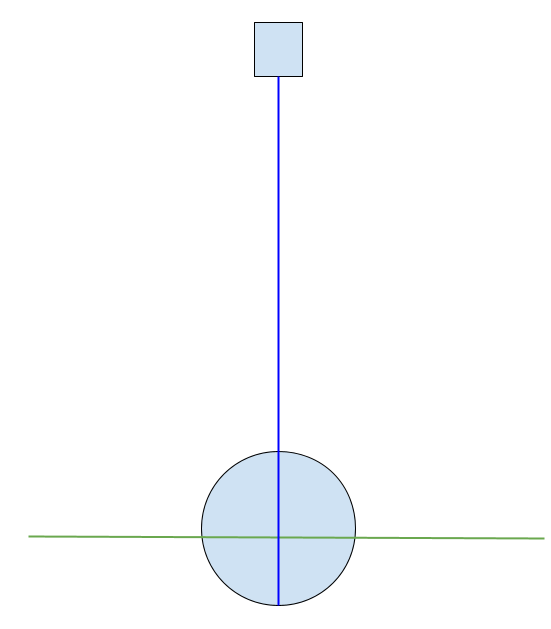
\includegraphics[width=0.4\linewidth]{../common/05_further_work/resources/00_genauigkeit_optimal.png}
    \caption{Optimale Genauigkeitsbestimmung}
    \label{fig:genauigkeit:optimal}
\end{figure}
Es ist offensichtlich, dass der Schnittpunkt des Strahls der Kamera aus mit der Ebene genau im Kugelzentrum liegt.
Wird nun angenommen, dass immer der reale Kugelmittelpunkt bestimmt werden kann, dann stimmt das Modell mit der Ebene
durch die Kugelzentren jedoch nicht mehr. Da die Kamera die Kugel aber immer weiter von der Seite sehen wird, je weiter diese am Rand
des Tischs liegt, wird diese zu einem Oval verzogen und es wird nicht mehr der reale Kugelmittelpunkt $M$ erkannt sondern ein Punkt $M'$
auf der Seite zur Kamera zugewandt. Das scheinbar optimale Verhalten sowie das reale ist in Abbildung \ref{fig:genauigkeit:real}
ersichtlich. Wie erkannt werden kann, ist die scheinbare Falscherkennung des Kugelmittelpunkts bei der Anwendung einer
Ebene auf Höhe des Kugelradius sogar von Vorteil, da die Fehlerdistanz zum realen Standort minimiert wird.
\begin{figure}[h!]
    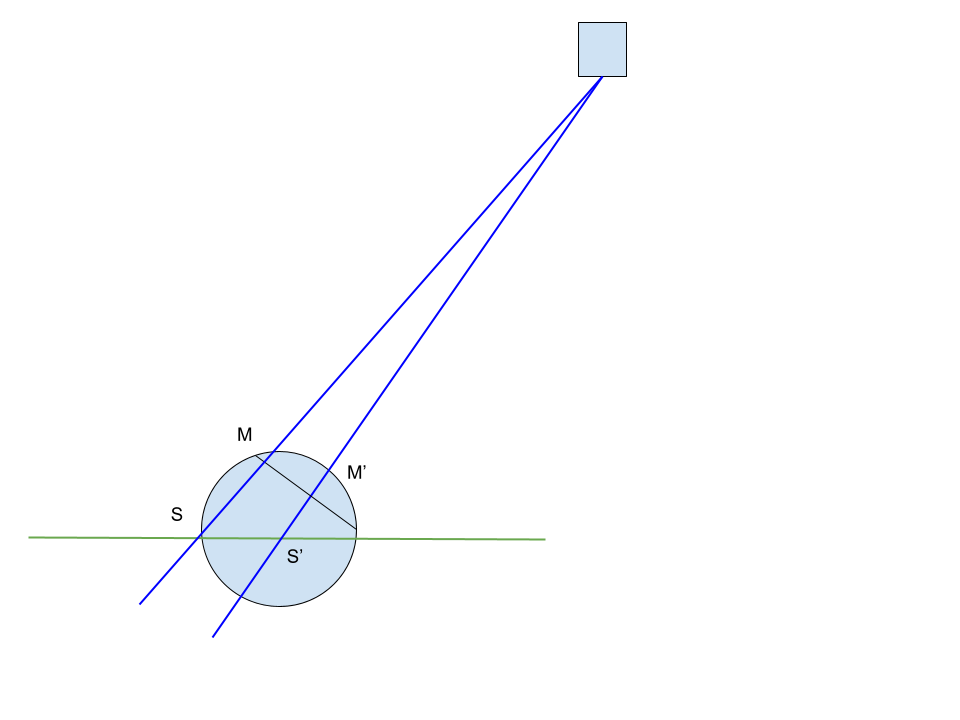
\includegraphics[width=0.4\linewidth]{../common/05_further_work/resources/01_genauigkeit_real.png}
    \caption{Reale Genauigkeitsbestimmung}
    \label{fig:genauigkeit:real}
\end{figure}


Nichtsdestotrotz kann es vonnöten sein, das Modell eventuell sogar der Realität entsprechend zu definieren, wenn erzielt
werden kann, dass immer der reale Kugelmittelpunkt gefunden wird. Weiterhin muss in diesem Zusammenhang zuerst ein genaueres
externes Messgerät gefunden werden, damit überhaupt eine Verbesserung der Genauigkeit nachgewiesen werden kann.


\end{document}
